%\pagebreak

\section{Thread mapping}

%What is mapping
The objective of \emph{thread mapping} or \emph{thread binding} is to define a
way to associate threads to physical processors. Once
mapped, the thread will stay on the processor during the execution without
being moved from one processor to another by the operating system. This is also
referred to as \emph{thread affinity}.

%Why mapping

A typical situation that needs thread mapping is shown in Figure
\ref{fig:mapping}, we have two dual core processors, each core is capable of
running two threads simultaneously. So the system can provide up to eight
\emph{physical threads} to an OpenMP application. 

In this system, suppose each processor core has its own L2 cache, and each CPU
core has its own L1 cache.

\begin{figure}[h!]
  \begin{center}
    \includegraphics[angle=0, width=0.45\textwidth]{mapping.eps}
    \caption{\footnotesize Thread mapping}
    \label{fig:mapping}
  \end{center}
\end{figure}

If an OpenMP application running on such system decides to use only four OpenMP
threads, then there are at least two mapping options one may choose from,

\begin{itemize} 

\item  let each CPU core have one OpenMP thread, so every processor core is
fully utilized. Or

\item let each CPU core have two OpenMP threads, leaving two CPUs idle. In this
way threads can share more data in cache among the adjacent ones.

\end{itemize}

It is hard to predict which mapping option can achieve better performance at an
abstract level. Depending on the hardware implementation and the program
itself, the answer may be different. So it will be desirable to let users
define the mapping to get better performance.

\subsection{Logical processors}

Before we define the actual mapping, it is important to think from an
application programmer's point of view, what kind of abstract view the hardware
system should look like.

A parallel program itself may be complicated enough that a regular user may not
want to know anything more than the number of processors offered in a system.
This is partially reflected in the current OpenMP standard. In \cite{Ope05}, an
API function \texttt{omp}\_\texttt{get}\_\\\texttt{num}\_\texttt{procs} returns
the number of the processors available to the program at the time the routine
is called. Most of the cases, it will be used to define the initial value for
the internal control variable \emph{nthreads-var}, which controls how many
threads are going to be created when a parallel region is encountered later on.

The environment variable \texttt{OMP\_NUM\_THREADS} and the API function
\texttt{omp\_set\_\\num\_threads} provide ways to change this control variable.
Yet in the current standard, there is no clear relationship between entities
represented by this control variable and the number returned from the function
\texttt{omp\_get\_num\_procs}, especially when the two values are different. 

The thread binding proposal we present here is to establish the affinity
relations between the \emph{OpenMP threads} controlled by the
\emph{nthreads-var} variable and the number of processors queried by
\texttt{omp\_get\_num\_procs}. In our proposal, we consider that the number
returned in the function \texttt{omp\_get\_num\_procs} is only for a
group of \emph{logical processors}. In Figure \ref{fig:mapping}, this number
can either be 4 or 8 depending whether the operating system made the extra
threads available. It is in contrast to the \emph{physical processors}, which
may be only 4 traditionally.

As an initial step, we will organize the logical processor group as a linear
array, giving each of them an id number, starting from 0, 1, and up to the
total number of the processors minus one.

Then the thread binding problem becomes the problem of having \emph{m}
OpenMP threads, and \emph{n} logical processor, how to assign those threads to
the processors, especially when $m \not= n$.

%Mapping define
\subsection{The mapping definition and its effect}

As explained above, we define the logical processors as a linear array. 

%We believe it is  
%enough complicated at this level that multi-dimension array is not needed. 

We use two environment variables to specify the first processor number that the
master thread binds to; and we specify the next processor number the second
thread will bind on with a "stride" on the processor array. 

For example, the following pair of environment variables

{\footnotesize
\begin{verbatim} 
    OMP_PROC_START=1; OMP_PROC_STRIDE=2
\end{verbatim}
}

will give us the mapping drawn in Figure \ref{fig:mapping}, where thread 0 is
on logical processor 1, thread 1 is on logical processor 3, and so on.  
We will use a \emph{round-robin} fashion to assign the other threads. 

%One way of
%defining it can be specified in the following pseudo code,

%{\footnotesize
%\begin{verbatim}
%    int num_Procs = omp_get_num_procs();
%    int num_Threads = omp_get_num_threads();
%
%    int start = getenv ("OMP_PROC_START");
%    int stride = getenv ("OMP_PROC_STRIDE");
%
%    int numPerRound = (num_Procs + stride -1 ) / stride;
%
%    for (int i = 0; i < num_Threads; i++) {
%      int round = i / numPerRound;
%      int count = i % numPerRound;
%
%      proc = (((start+round)+ stride * count)) % num_Procs;
%
%      // Assign thread i on processor proc
%      // This will be OS specific
%      ...
%    }
%\end{verbatim}
%}

%The round-robin method we used is always shifting one further from the start
%position in the previous round. Other alternatives are possible.

% Real example

\begin{figure}[h!]
  \begin{center}
    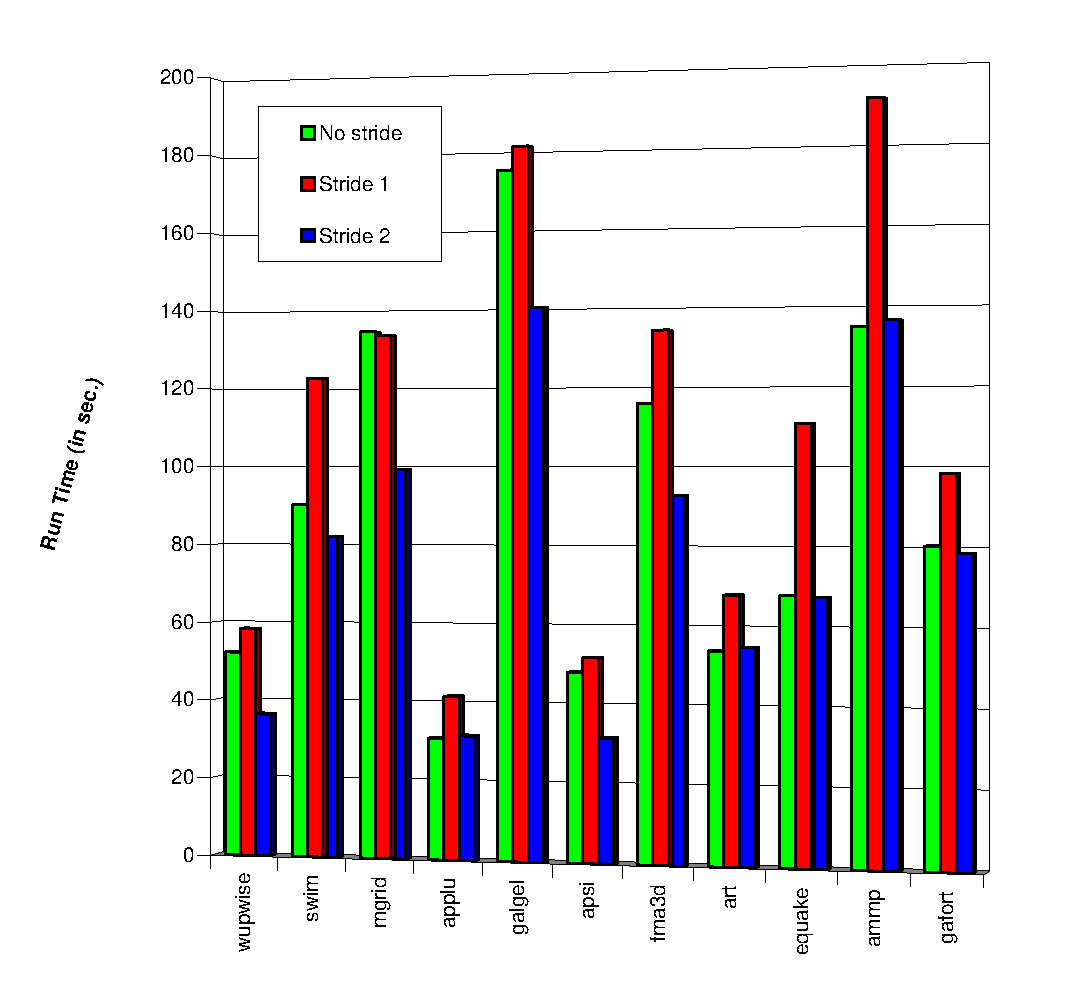
\includegraphics[angle=0, width=0.60\textwidth]{specomp.eps}
    \caption{\footnotesize SPEC OMP performance}
    \label{fig:specomp}
  \end{center}
\end{figure}

We used SPEC OpenMP benchmark to demonstrate the performance impact of thread
mapping. In Figure \ref{fig:specomp}, a 64 processor core POWER5 machine is used to
measure the OpenMP suite. The SMT option of POWER5 was on. So each processor is
capable of running two threads.  We set \texttt{OMP\_NUM\_THREADS} to be 64,
and compared the following situations

\begin{itemize}
    
  \item No processor mapping specification.

  \item Stride as one by \texttt{OMP\_PROC\_START=0; OMP\_PROC\_STRIDE=1}, and

  \item Stride as two by \texttt{OMP\_PROC\_START=0; OMP\_PROC\_STRIDE=2}

\end{itemize}

The rest of the execution environment, including compilation flags, are all the
same. From the figure, one can see that stride two setting has the best overall
performance numbers; Stride one setting is the worst: No stride setting is in
between.  And some of the difference can be as big as 40\%, such as in
equak, apsi and wupwise.


\subsection{More about the mapping}

In the mapping scheme above, all the processors and threads are kept in a
simple linear relation. More complicated mapping may be achieved though other
structures. For example, we can define a arbitrary mapping as an integer array.
We are not sure that such level of complexity is useful. We will see that more
complicated mapping actually can be achieved in the next section when we extend
the logical processor array to a \emph{processor group}.

We also need to point out that the mapping we defined here is only the one from
the OpenMP threads to the logical processors. We did not define how logical
processors mapped to physical threads. It is left as an implementation defined
issue. 

%For example, if the operating system is different, this mapping will be
%different.



%In our experiment, we have tested on AIX and Linux on POWER system.

%Even in this simple format
%Linux has special way of naming processors

%Merging two physical processors into one
%this is cell, extra thing needed? 
%at least access shared variable is complicated.

%As a summary, we did not involve nested parallelism and thread grouping in this
%first step.  Yet more complicated mapping options introduced in the next
%section will be considered as a natural extension of what we discussed here.



